\documentclass[]{article}
\usepackage{lmodern}
\usepackage{amssymb,amsmath}
\usepackage{ifxetex,ifluatex}
\usepackage{fixltx2e} % provides \textsubscript
\ifnum 0\ifxetex 1\fi\ifluatex 1\fi=0 % if pdftex
  \usepackage[T1]{fontenc}
  \usepackage[utf8]{inputenc}
\else % if luatex or xelatex
  \ifxetex
    \usepackage{mathspec}
  \else
    \usepackage{fontspec}
  \fi
  \defaultfontfeatures{Ligatures=TeX,Scale=MatchLowercase}
\fi
% use upquote if available, for straight quotes in verbatim environments
\IfFileExists{upquote.sty}{\usepackage{upquote}}{}
% use microtype if available
\IfFileExists{microtype.sty}{%
\usepackage{microtype}
\UseMicrotypeSet[protrusion]{basicmath} % disable protrusion for tt fonts
}{}
\usepackage[margin=1in]{geometry}
\usepackage{hyperref}
\hypersetup{unicode=true,
            pdftitle={Activity monitoring data analysis},
            pdfauthor={Kidpea LAU},
            pdfborder={0 0 0},
            breaklinks=true}
\urlstyle{same}  % don't use monospace font for urls
\usepackage{color}
\usepackage{fancyvrb}
\newcommand{\VerbBar}{|}
\newcommand{\VERB}{\Verb[commandchars=\\\{\}]}
\DefineVerbatimEnvironment{Highlighting}{Verbatim}{commandchars=\\\{\}}
% Add ',fontsize=\small' for more characters per line
\usepackage{framed}
\definecolor{shadecolor}{RGB}{248,248,248}
\newenvironment{Shaded}{\begin{snugshade}}{\end{snugshade}}
\newcommand{\KeywordTok}[1]{\textcolor[rgb]{0.13,0.29,0.53}{\textbf{#1}}}
\newcommand{\DataTypeTok}[1]{\textcolor[rgb]{0.13,0.29,0.53}{#1}}
\newcommand{\DecValTok}[1]{\textcolor[rgb]{0.00,0.00,0.81}{#1}}
\newcommand{\BaseNTok}[1]{\textcolor[rgb]{0.00,0.00,0.81}{#1}}
\newcommand{\FloatTok}[1]{\textcolor[rgb]{0.00,0.00,0.81}{#1}}
\newcommand{\ConstantTok}[1]{\textcolor[rgb]{0.00,0.00,0.00}{#1}}
\newcommand{\CharTok}[1]{\textcolor[rgb]{0.31,0.60,0.02}{#1}}
\newcommand{\SpecialCharTok}[1]{\textcolor[rgb]{0.00,0.00,0.00}{#1}}
\newcommand{\StringTok}[1]{\textcolor[rgb]{0.31,0.60,0.02}{#1}}
\newcommand{\VerbatimStringTok}[1]{\textcolor[rgb]{0.31,0.60,0.02}{#1}}
\newcommand{\SpecialStringTok}[1]{\textcolor[rgb]{0.31,0.60,0.02}{#1}}
\newcommand{\ImportTok}[1]{#1}
\newcommand{\CommentTok}[1]{\textcolor[rgb]{0.56,0.35,0.01}{\textit{#1}}}
\newcommand{\DocumentationTok}[1]{\textcolor[rgb]{0.56,0.35,0.01}{\textbf{\textit{#1}}}}
\newcommand{\AnnotationTok}[1]{\textcolor[rgb]{0.56,0.35,0.01}{\textbf{\textit{#1}}}}
\newcommand{\CommentVarTok}[1]{\textcolor[rgb]{0.56,0.35,0.01}{\textbf{\textit{#1}}}}
\newcommand{\OtherTok}[1]{\textcolor[rgb]{0.56,0.35,0.01}{#1}}
\newcommand{\FunctionTok}[1]{\textcolor[rgb]{0.00,0.00,0.00}{#1}}
\newcommand{\VariableTok}[1]{\textcolor[rgb]{0.00,0.00,0.00}{#1}}
\newcommand{\ControlFlowTok}[1]{\textcolor[rgb]{0.13,0.29,0.53}{\textbf{#1}}}
\newcommand{\OperatorTok}[1]{\textcolor[rgb]{0.81,0.36,0.00}{\textbf{#1}}}
\newcommand{\BuiltInTok}[1]{#1}
\newcommand{\ExtensionTok}[1]{#1}
\newcommand{\PreprocessorTok}[1]{\textcolor[rgb]{0.56,0.35,0.01}{\textit{#1}}}
\newcommand{\AttributeTok}[1]{\textcolor[rgb]{0.77,0.63,0.00}{#1}}
\newcommand{\RegionMarkerTok}[1]{#1}
\newcommand{\InformationTok}[1]{\textcolor[rgb]{0.56,0.35,0.01}{\textbf{\textit{#1}}}}
\newcommand{\WarningTok}[1]{\textcolor[rgb]{0.56,0.35,0.01}{\textbf{\textit{#1}}}}
\newcommand{\AlertTok}[1]{\textcolor[rgb]{0.94,0.16,0.16}{#1}}
\newcommand{\ErrorTok}[1]{\textcolor[rgb]{0.64,0.00,0.00}{\textbf{#1}}}
\newcommand{\NormalTok}[1]{#1}
\usepackage{graphicx,grffile}
\makeatletter
\def\maxwidth{\ifdim\Gin@nat@width>\linewidth\linewidth\else\Gin@nat@width\fi}
\def\maxheight{\ifdim\Gin@nat@height>\textheight\textheight\else\Gin@nat@height\fi}
\makeatother
% Scale images if necessary, so that they will not overflow the page
% margins by default, and it is still possible to overwrite the defaults
% using explicit options in \includegraphics[width, height, ...]{}
\setkeys{Gin}{width=\maxwidth,height=\maxheight,keepaspectratio}
\IfFileExists{parskip.sty}{%
\usepackage{parskip}
}{% else
\setlength{\parindent}{0pt}
\setlength{\parskip}{6pt plus 2pt minus 1pt}
}
\setlength{\emergencystretch}{3em}  % prevent overfull lines
\providecommand{\tightlist}{%
  \setlength{\itemsep}{0pt}\setlength{\parskip}{0pt}}
\setcounter{secnumdepth}{0}
% Redefines (sub)paragraphs to behave more like sections
\ifx\paragraph\undefined\else
\let\oldparagraph\paragraph
\renewcommand{\paragraph}[1]{\oldparagraph{#1}\mbox{}}
\fi
\ifx\subparagraph\undefined\else
\let\oldsubparagraph\subparagraph
\renewcommand{\subparagraph}[1]{\oldsubparagraph{#1}\mbox{}}
\fi

%%% Use protect on footnotes to avoid problems with footnotes in titles
\let\rmarkdownfootnote\footnote%
\def\footnote{\protect\rmarkdownfootnote}

%%% Change title format to be more compact
\usepackage{titling}

% Create subtitle command for use in maketitle
\newcommand{\subtitle}[1]{
  \posttitle{
    \begin{center}\large#1\end{center}
    }
}

\setlength{\droptitle}{-2em}

  \title{Activity monitoring data analysis}
    \pretitle{\vspace{\droptitle}\centering\huge}
  \posttitle{\par}
    \author{Kidpea LAU}
    \preauthor{\centering\large\emph}
  \postauthor{\par}
      \predate{\centering\large\emph}
  \postdate{\par}
    \date{25/09/2018}


\begin{document}
\maketitle

\section{About the data:}\label{about-the-data}

The data from a personal activity monitoring device. This device
collects data at 5 minute intervals through out the day. The data
consists of two months of data from an anonymous individual collected
during the months of October and November, 2012 and include the number
of steps taken in 5 minute intervals each day.

\section{load the data}\label{load-the-data}

\begin{Shaded}
\begin{Highlighting}[]
\NormalTok{fileUrl<-}\StringTok{"https://d396qusza40orc.cloudfront.net/repdata%2Fdata%2Factivity.zip"}
\KeywordTok{download.file}\NormalTok{(fileUrl,}\DataTypeTok{destfile=}\StringTok{"./data1/Dataset.zip"}\NormalTok{)}
\KeywordTok{unzip}\NormalTok{(}\DataTypeTok{zipfile=}\StringTok{"./data1/Dataset.zip"}\NormalTok{,}\DataTypeTok{exdir=}\StringTok{"./data1"}\NormalTok{)}
\NormalTok{path_rf <-}\StringTok{ }\KeywordTok{file.path}\NormalTok{(}\StringTok{"./data1"}\NormalTok{ , }\StringTok{"data1.csv"}\NormalTok{)}
\NormalTok{files<-}\KeywordTok{list.files}\NormalTok{(path_rf, }\DataTypeTok{recursive=}\OtherTok{TRUE}\NormalTok{)}
\NormalTok{act<-}\KeywordTok{read.csv}\NormalTok{(}\StringTok{"./data1/activity.csv"}\NormalTok{)}
\end{Highlighting}
\end{Shaded}

\section{Histogram of the total number of steps taken each
day}\label{histogram-of-the-total-number-of-steps-taken-each-day}

\begin{Shaded}
\begin{Highlighting}[]
\NormalTok{stepperday<-}\KeywordTok{tapply}\NormalTok{(act}\OperatorTok{$}\NormalTok{steps,act}\OperatorTok{$}\NormalTok{date,sum,}\DataTypeTok{na.rm=}\NormalTok{T)}
\KeywordTok{hist}\NormalTok{(stepperday, }\DataTypeTok{xlab =} \StringTok{"number of steps"}\NormalTok{,}
     \DataTypeTok{main =} \StringTok{"the total number of steps taken each day"}\NormalTok{)}
\end{Highlighting}
\end{Shaded}

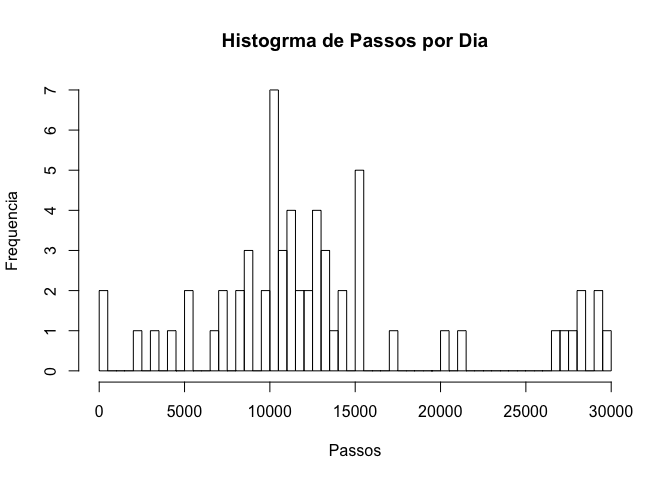
\includegraphics{md_files/figure-latex/unnamed-chunk-1-1.pdf}

\section{Mean and median number of steps taken each
day}\label{mean-and-median-number-of-steps-taken-each-day}

\begin{Shaded}
\begin{Highlighting}[]
\KeywordTok{summary}\NormalTok{(stepperday)}
\end{Highlighting}
\end{Shaded}

\begin{verbatim}
##    Min. 1st Qu.  Median    Mean 3rd Qu.    Max. 
##       0    6778   10395    9354   12811   21194
\end{verbatim}

\section{Time series plot of the average number of steps
taken}\label{time-series-plot-of-the-average-number-of-steps-taken}

\begin{Shaded}
\begin{Highlighting}[]
\NormalTok{mean_interval <-}\StringTok{ }\KeywordTok{tapply}\NormalTok{(act}\OperatorTok{$}\NormalTok{steps, act}\OperatorTok{$}\NormalTok{interval, mean, }\DataTypeTok{na.rm =}\NormalTok{ T)}

\KeywordTok{plot}\NormalTok{(mean_interval, }\DataTypeTok{type =} \StringTok{"l"}\NormalTok{, }\DataTypeTok{main =} \StringTok{"time series plot"}\NormalTok{, }\DataTypeTok{xlab =} \StringTok{"the 5-minute interval"}\NormalTok{, }\DataTypeTok{ylab =} \StringTok{"the average number of steps"}\NormalTok{)}
\end{Highlighting}
\end{Shaded}

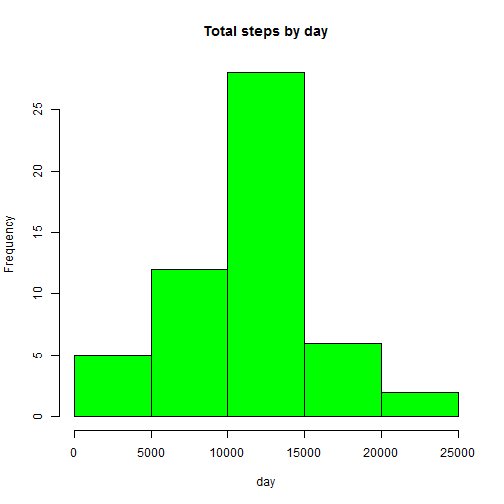
\includegraphics{md_files/figure-latex/unnamed-chunk-3-1.pdf}

\section{The 5-minute interval that, on average, contains the maximum
number of
steps}\label{the-5-minute-interval-that-on-average-contains-the-maximum-number-of-steps}

\begin{Shaded}
\begin{Highlighting}[]
\KeywordTok{which.max}\NormalTok{(mean_interval)}
\end{Highlighting}
\end{Shaded}

\begin{verbatim}
## 835 
## 104
\end{verbatim}

\section{Code to describe and show a strategy for imputing missing
data}\label{code-to-describe-and-show-a-strategy-for-imputing-missing-data}

\begin{Shaded}
\begin{Highlighting}[]
\NormalTok{stepsNA <-}\StringTok{ }\KeywordTok{sum}\NormalTok{(}\KeywordTok{is.na}\NormalTok{(act}\OperatorTok{$}\NormalTok{steps))}
\NormalTok{dateNA <-}\StringTok{ }\KeywordTok{sum}\NormalTok{(}\KeywordTok{is.na}\NormalTok{(act}\OperatorTok{$}\NormalTok{date))}
\NormalTok{intervalNA <-}\StringTok{ }\KeywordTok{sum}\NormalTok{(}\KeywordTok{is.na}\NormalTok{(act}\OperatorTok{$}\NormalTok{interval))}
\end{Highlighting}
\end{Shaded}

\section{Histogram of the total number of steps taken each day after
missing values are
imputed}\label{histogram-of-the-total-number-of-steps-taken-each-day-after-missing-values-are-imputed}

\begin{Shaded}
\begin{Highlighting}[]
\NormalTok{numMissingValues <-}\StringTok{ }\KeywordTok{length}\NormalTok{(}\KeywordTok{which}\NormalTok{(}\KeywordTok{is.na}\NormalTok{(act}\OperatorTok{$}\NormalTok{steps)))}
\NormalTok{numMissingValues}
\end{Highlighting}
\end{Shaded}

\begin{verbatim}
## [1] 2304
\end{verbatim}

\subsubsection{set a function to impute the
NA}\label{set-a-function-to-impute-the-na}

\begin{Shaded}
\begin{Highlighting}[]
\NormalTok{impute <-}\StringTok{ }\ControlFlowTok{function}\NormalTok{(x, x.impute)\{}\KeywordTok{ifelse}\NormalTok{(}\KeywordTok{is.na}\NormalTok{(x),x.impute,x)\}}
\NormalTok{act2 <-}\StringTok{ }\NormalTok{act}
\NormalTok{act2}\OperatorTok{$}\NormalTok{steps <-}\StringTok{ }\KeywordTok{impute}\NormalTok{(act}\OperatorTok{$}\NormalTok{steps, }\KeywordTok{mean}\NormalTok{(act}\OperatorTok{$}\NormalTok{steps))}
\end{Highlighting}
\end{Shaded}

\subsubsection{Make a histogram of the total number of steps taken each
day}\label{make-a-histogram-of-the-total-number-of-steps-taken-each-day}

\begin{Shaded}
\begin{Highlighting}[]
\NormalTok{act2step <-}\StringTok{ }\KeywordTok{tapply}\NormalTok{(act2}\OperatorTok{$}\NormalTok{steps, act2}\OperatorTok{$}\NormalTok{date, sum,}\DataTypeTok{na.rm=}\OtherTok{TRUE}\NormalTok{)}
\KeywordTok{hist}\NormalTok{(act2step, }\DataTypeTok{xlab=}\StringTok{'Total steps per day (Imputed)'}\NormalTok{,}\DataTypeTok{bins=}\DecValTok{50}\NormalTok{)}
\end{Highlighting}
\end{Shaded}

\begin{verbatim}
## Warning in plot.window(xlim, ylim, "", ...): "bins"不是图形参数
\end{verbatim}

\begin{verbatim}
## Warning in title(main = main, sub = sub, xlab = xlab, ylab = ylab, ...):
## "bins"不是图形参数
\end{verbatim}

\begin{verbatim}
## Warning in axis(1, ...): "bins"不是图形参数
\end{verbatim}

\begin{verbatim}
## Warning in axis(2, ...): "bins"不是图形参数
\end{verbatim}

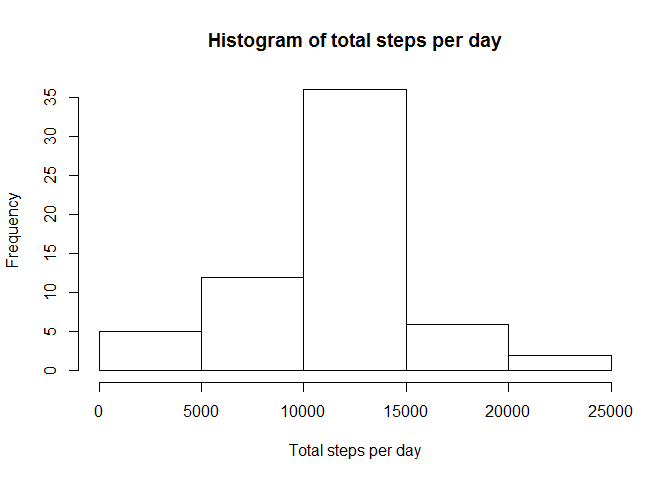
\includegraphics{md_files/figure-latex/unnamed-chunk-8-1.pdf}

\section{Panel plot comparing the average number of steps taken per
5-minute interval across weekdays and
weekends}\label{panel-plot-comparing-the-average-number-of-steps-taken-per-5-minute-interval-across-weekdays-and-weekends}

\subsection{make a new vector to describe weekday and
weekend}\label{make-a-new-vector-to-describe-weekday-and-weekend}

\begin{Shaded}
\begin{Highlighting}[]
\NormalTok{act2}\OperatorTok{$}\NormalTok{dateType <-}\StringTok{  }\KeywordTok{ifelse}\NormalTok{(}\KeywordTok{as.POSIXlt}\NormalTok{(act2}\OperatorTok{$}\NormalTok{date)}\OperatorTok{$}\NormalTok{wday }\OperatorTok\StringTok{ }\KeywordTok{c}\NormalTok{(}\DecValTok{0}\NormalTok{,}\DecValTok{6}\NormalTok{), }\StringTok{'weekend'}\NormalTok{, }\StringTok{'weekday'}\NormalTok{)}
\end{Highlighting}
\end{Shaded}

\subsection{make the plot}\label{make-the-plot}

\begin{Shaded}
\begin{Highlighting}[]
\KeywordTok{library}\NormalTok{(ggplot2)}
\NormalTok{avgAct2 <-}\StringTok{ }\KeywordTok{aggregate}\NormalTok{(steps }\OperatorTok{~}\StringTok{ }\NormalTok{interval }\OperatorTok{+}\StringTok{ }\NormalTok{dateType, }\DataTypeTok{data=}\NormalTok{act2, mean)}
\KeywordTok{ggplot}\NormalTok{(avgAct2, }\KeywordTok{aes}\NormalTok{(interval, steps)) }\OperatorTok{+}\StringTok{ }
\StringTok{  }\KeywordTok{geom_line}\NormalTok{() }\OperatorTok{+}\StringTok{ }
\StringTok{  }\KeywordTok{facet_grid}\NormalTok{(dateType }\OperatorTok{~}\StringTok{ }\NormalTok{.) }\OperatorTok{+}
\StringTok{  }\KeywordTok{xlab}\NormalTok{(}\StringTok{"5-minute interval"}\NormalTok{) }\OperatorTok{+}\StringTok{ }
\StringTok{  }\KeywordTok{ylab}\NormalTok{(}\StringTok{"avarage number of steps"}\NormalTok{)}
\end{Highlighting}
\end{Shaded}

\includegraphics{md_files/figure-latex/scatterplot-1.pdf}


\end{document}
